%%%%%%%%%%%%%%%%%%%%%%%%%%%%%%%%%%%%%%%%%%  不使用 authblk 包制作标题  %%%%%%%%%%%%%%%%%%%%%%%%%%%%%%%%%%%%%%%%%%%%%%
%-------------------------------PPT Title-------------------------------------
\title{{\rm LAMMPS}算例举要}
%-----------------------------------------------------------------------------
%----------------------------Author & Date------------------------------------

%\author[\textrm{Jun\_Jiang}]{姜\;\;骏\inst{}} %[]{} (optional, use only with lots of authors)
%% - Give the names in the same order as the appear in the paper.
%% - Use the \inst{?} command only if the authors have different
%%   affiliation.
\institute[BCC]{\inst{}%
%\institute[Gain~Strong]{\inst{}%
\vskip -20pt 北京市计算中心~云平台事业部~~姜骏}
%\vskip -20pt {\large 格致斯创~科技}}
\date[\today] % (optional, should be abbreviation of conference name)
{%	{\fontsize{6.2pt}{4.2pt}\selectfont{\textcolor{blue}{E-mail:~}\url{jiangjun@bcc.ac.cn}}}
\vskip 45 pt {\fontsize{8.2pt}{6.2pt}\selectfont{%清华大学\;\;物理系% 报告地点
	\vskip 5 pt \textrm{2023.11.23-24}}}
}

%% - Either use conference name or its abbreviation
%% - Not really information to the audience, more for people (including
%%   yourself) who are reading the slides onlin%%   yourself) who are reading the slides onlin%%   yourself) who are reading the slides onlineee
%%%%%%%%%%%%%%%%%%%%%%%%%%%%%%%%%%%%%%%%%%%%%%%%%%%%%%%%%%%%%%%%%%%%%%%%%%%%%%%%%%%%%%%%%%%%%%%%%%%%%%%%%%%%%%%%%%%%%

\subject{}
% This is only inserted into the PDF information catalog. Can be left
% out.
%\maketitle
\frame
{
%	\frametitle{\fontsize{9.5pt}{5.2pt}\selectfont{\textcolor{orange}{“高通量并发式材料计算算法与软件”年度检查}}}
\titlepage
}
%-----------------------------------------------------------------------------

%------------------------------------------------------------------------------列出全文 outline ---------------------------------------------------------------------------------
\section{基本计算}\label{Sec:General}
%真空中的孤立原子的基态能量是\textrm{VASP}中最简单的算例,通过学习金属\textrm{Pt}原子基态能量的计算,可以掌握典型的\textrm{VASP}的主体流程\footnote{在所有计算之前,请确认\textrm{VASP}软件已经正确安装。},了解体系基态能量最小化的基本算法,并熟悉基本的输入/输出文件的内容。此外,还可以了解如何在已完成计算的基础上,进行计算精度提升或完成后续计算等一系列处理方式。
%\subsection{输入文件}
\frame
{
	\frametitle{\textrm{LAMMPS}一般计算流程}
\begin{figure}[h!]
\centering
\vskip -5pt
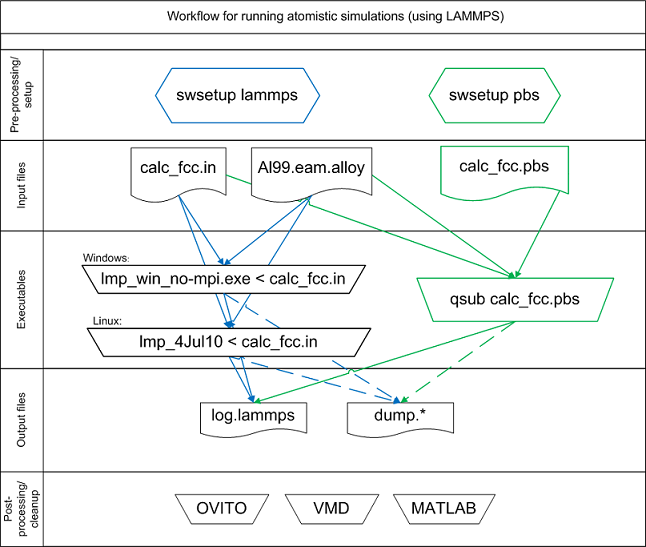
\includegraphics[height=2.50in,width=3.0in, viewport=0 0 646 547,clip]{Lammps_workflow.png}
\caption{\fontsize{6.2pt}{5.2pt}\selectfont{\textrm{The general workflow for running molecular dynamics simulations using LAMMPS.}}}%(与文献\cite{EPJB33-47_2003}图1对比)
\label{General_Workflow}
\end{figure}
}

\frame
{
	\frametitle{\textrm{LAMMPS}的输入参数说明}
	{\fontsize{7.5pt}{4.0pt}\selectfont{
%\verbatiminput{Figures/Lammps_in_lj.txt} %为保险:~选用文件名绝对路径
\verbatiminput{Figures/Lammps_tutorial-01-in_01.txt} %为保险:~选用文件名绝对路径
}
\begin{itemize}
	\item \textcolor{cyan}{\textit{\#}}~开头的部分表示注释,\textrm{LAMMPS}不作任何处理
\end{itemize}
}
\vskip 5pt
%\textrm{LAMMPS}模拟的初始化
{\fontsize{7.5pt}{4.0pt}\selectfont{
%\verbatiminput{Figures/Lammps_in_lj.txt} %为保险:~选用文件名绝对路径
\verbatiminput{Figures/Lammps_tutorial-01-in_02.txt} %为保险:~选用文件名绝对路径
}
\begin{itemize}
	\item \textcolor{cyan}{\textit{clear}}:~清除全部内存信息
	\item \textcolor{cyan}{\textit{unit}}:~设定模拟的单位~ (\textcolor{blue}{\textrm{metal}}~表示选择\textrm{\AA}和\textrm{eV}为单位)
	\item \textcolor{cyan}{\textit{dimension}}:~设定模拟维度~:~\textcolor{blue}{\textrm{3}}~表示三维模拟
	\item \textcolor{cyan}{\textit{boundary}}~\textcolor{blue}{\textrm{p~p~p}}:~表示在$x$-,$y$-,$z$-方向采用周期性边界条件
		\begin{itemize}
{\fontsize{6.2pt}{4.0pt}\selectfont{
			\item \textrm{p}:~周期性边界条件\textrm{(periodic)}
			\item \textrm{f}:~非周期性固定边界条件\textrm{(fixed)}
			\item \textrm{s}:~非周期性包覆边界条件\textrm{(shrink-wrapped)}
			\item \textrm{m}:~非周期性包覆最小值边界条件\textrm{(minimum value)}}}
		\end{itemize}
\end{itemize}
}
}

\frame
{
	\frametitle{\textrm{LAMMPS}的输入参数说明}
	{\fontsize{7.5pt}{4.0pt}\selectfont{
%\verbatiminput{Figures/Lammps_in_lj.txt} %为保险:~选用文件名绝对路径
\verbatiminput{Figures/Lammps_tutorial-01-in_03.txt} %为保险:~选用文件名绝对路径
}
\begin{itemize}
	\item \textcolor{cyan}{\textit{lattice}}:~设定晶格信息~(可选择的晶格类型有\textrm{sc, fcc, bcc, hcp, diamond}等)、\\
		晶格常数(数值\textrm{4})、晶格矢量方向等
	\item \textcolor{cyan}{\textit{region}}:~设定模拟的原胞,此处设定模拟的名为\textcolor{blue}{\textrm{box}}的\textrm{block}(可以理解为原胞)采用晶格单位,并要求\textrm{box}每个方向的大小取为一个晶格常数
	\item \textcolor{cyan}{\textit{create\_box}}:~使用\textcolor{cyan}{\textit{region}}确定的参数构建模拟的\textrm{box},数量为\textcolor{red}{1个}
	\item \textcolor{cyan}{\textit{replicate}}:~设定每个方向上重复的元胞数目
\end{itemize}
}
%\textrm{LAMMPS}模拟的初始化
{\fontsize{7.5pt}{4.0pt}\selectfont{
%\verbatiminput{Figures/Lammps_in_lj.txt} %为保险:~选用文件名绝对路径
\verbatiminput{Figures/Lammps_tutorial-01-in_04.txt} %为保险:~选用文件名绝对路径
}
\begin{itemize}
	\item \textcolor{cyan}{\textit{pair\_style}}:~设定原子间相互作用(力场)类型
	\item \textcolor{cyan}{\textit{pair\_coeff}}~\textrm{metal}:~设定相互作用势(力场)的系数\\
		{\fontsize{6.2pt}{5.2pt}\selectfont{\textcolor{magenta}{势函数(力场)的扩展名提示的是使用相互作用的类型}}}
	\item \textcolor{cyan}{\textit{neighbor}}:~设置表面距离
	\item \textcolor{cyan}{\textit{neigh\_modify}}:~设置原子运动
\end{itemize}
}
}

\frame
{
	\frametitle{\textrm{LAMMPS}的输入参数说明}
	{\fontsize{7.5pt}{4.0pt}\selectfont{
%\verbatiminput{Figures/Lammps_in_lj.txt} %为保险:~选用文件名绝对路径
\verbatiminput{Figures/Lammps_tutorial-01-in_05.txt} %为保险:~选用文件名绝对路径
}
\begin{itemize}
	\item \textcolor{cyan}{\textit{compute}}:~定义计算变量:\\
		\begin{enumerate}
{\fontsize{7.5pt}{4.0pt}\selectfont{
			\item \textcolor{purple}{变量\textrm{eng}}:~定义为平均每个原子的势能
			\item \textcolor{purple}{变量\textrm{eatom}}:~定义为求和全部\textcolor{purple}{变量\textrm{eng}}的值:~\textcolor{blue}{\textrm{reduce}}~表示减(负)}}
		\end{enumerate}
\end{itemize}
}
}

\frame
{
	\frametitle{\textrm{LAMMPS}的输入参数说明}
%\vskip 5pt
%\textrm{LAMMPS}模拟的初始化
{\fontsize{7.5pt}{4.0pt}\selectfont{
%\verbatiminput{Figures/Lammps_in_lj.txt} %为保险:~选用文件名绝对路径
\verbatiminput{Figures/Lammps_tutorial-01-in_06.txt} %为保险:~选用文件名绝对路径
}
\begin{itemize}
	\item \textcolor{cyan}{\textit{reset\_timestep}}:~设定模拟步数归零\footnote{\fontsize{6.2pt}{5.2pt}\selectfont{\textrm{LAMMPS}模拟中,一般需要设置能量最小化、弛豫、数据采集等阶段,不同阶段模拟步数不同。默认情况下,模拟步数是从模拟开始到模拟结束一直累加计算的}}
	\item \textcolor{cyan}{\textit{fix}}:~设定\textrm{box/relax},能量最小化过程中对模拟盒施外压,各向同性\textrm{(iso)}都弛豫到\textrm{0.0~Pa}:~\textcolor{blue}{\textrm{vmax}}:~正压压缩,负压膨胀
	\item \textcolor{cyan}{\textit{thermo}}:~每运行\textcolor{blue}{10}次在屏幕上输出一次运行结果
	\item \textcolor{cyan}{\textit{thermo\_style}}:~设定屏幕输出信息
	\item \textcolor{cyan}{\textit{min\_style}}:~设定优化算法(最小化算法),\textcolor{blue}{\textrm{cg}}~指定共轭梯度法
	\item \textcolor{cyan}{\textit{minimize}}:~设定开始最小化过程和最小化收敛精度和最大迭代次数:\\
		其中1,3项为能量最小化,2,4项为能量梯度(力)\\
		原胞弛豫的模拟由晶格常数为\textrm{4\AA}到\textrm{4.05\AA}
\end{itemize}
}
}

\frame
{
	\frametitle{\textrm{LAMMPS}的输入参数说明}
	{\fontsize{7.5pt}{4.0pt}\selectfont{
%\verbatiminput{Figures/Lammps_in_lj.txt} %为保险:~选用文件名绝对路径
\verbatiminput{Figures/Lammps_tutorial-01-in_07.txt} %为保险:~选用文件名绝对路径
}
\begin{itemize}
	\item \textcolor{cyan}{\textit{natoms}}:~变量定义所有原子数
	\item \textcolor{cyan}{\textit{teng}}:~变量定义总的势能:~\textcolor{blue}{\textrm{teng=eatoms}}
	\item \textcolor{cyan}{\textit{length}}:~变量定义模拟原胞长度:~\textcolor{blue}{\textrm{length=lx}}(模拟盒$x$方向为例)
	\item \textcolor{cyan}{\textit{ecoh}}:~变量定义内聚能:~\textcolor{blue}{\textrm{ecoh=v\_teng/v\_natoms}}\footnote{\fontsize{6.2pt}{5.2pt}\selectfont{同一语句中出现多个变量引用时用\textrm{\textcolor{red}{v}\_variable}表示}}
\end{itemize}}
%\textrm{LAMMPS}模拟的初始化
{\fontsize{7.5pt}{4.0pt}\selectfont{
%\verbatiminput{Figures/Lammps_in_lj.txt} %为保险:~选用文件名绝对路径
\verbatiminput{Figures/Lammps_tutorial-01-in_08.txt} %为保险:~选用文件名绝对路径
}
\begin{itemize}
	\item 设定屏幕输出和\textrm{log}文件的输出变量
	\item \textcolor{red}{\$\{\}}表示定义变量的引用
\end{itemize}
}
}

%\frame[allowframebreaks]
%{
%	\frametitle{\textrm{LAMMPS}的输入文件}
%\fontsize{6.0pt}{4.0pt}\selectfont{
%%\verbatiminput{Figures/Lammps_in_lj.txt} %为保险:~选用文件名绝对路径
%\verbatiminput{Figures/Lammps_tutorial-01-Lammps-in.txt} %为保险:~选用文件名绝对路径
%}
%}
%
\frame
{
	\frametitle{\textrm{LAMMPS}的输出结果}
	\textrm{LAMMPS}执行命令:
	\vskip 5pt
	\textcolor{blue}{lmp}~\textcolor{magenta}{-in}~calc\_fcc.in
	\vskip 5pt
\begin{figure}[h!]
\centering
\vskip -5pt
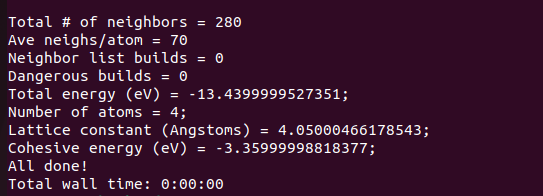
\includegraphics[height=1.50in,width=4.0in, viewport=0 0 543 196,clip]{Lammps_output.png}
\caption{\fontsize{6.2pt}{5.2pt}\selectfont{\textrm{The end of the logfile/screen output using LAMMPS.}}}%(与文献\cite{EPJB33-47_2003}图1对比)
\label{LAMMPS_output}
\end{figure}
}

\frame[allowframebreaks]
{
	\frametitle{\textrm{LAMMPS}的输入文件}
	{\fontsize{6.0pt}{4.0pt}\selectfont{
%\verbatiminput{Figures/Lammps_in_lj.txt} %为保险:~选用文件名绝对路径
\verbatiminput{Figures/Lammps_tutorial-02-in.txt} %为保险:~选用文件名绝对路径
}}
	\textrm{LAMMPS}执行命令:
	\vskip 5pt
	\textcolor{blue}{lmp}~\textcolor{magenta}{-in}~calc\_fcc.in~\textcolor{red}{-var~latconst~4}
}

\frame[allowframebreaks]
{
	\frametitle{\textrm{LAMMPS}的输入文件:~基于\textrm{Matlab}的执行}
	{\fontsize{6.0pt}{4.0pt}\selectfont{
%\verbatiminput{Figures/Lammps_in_lj.txt} %为保险:~选用文件名绝对路径
\verbatiminput{Figures/Lammps_tutorial-02-Lammps-in.txt} %为保险:~选用文件名绝对路径
}}
}

\frame[allowframebreaks]
{
	\frametitle{\textrm{LAMMPS}的输入文件:~基于\textrm{Matlab}的执行}
	{\fontsize{6.0pt}{4.0pt}\selectfont{
%\verbatiminput{Figures/Lammps_in_lj.txt} %为保险:~选用文件名绝对路径
\verbatiminput{Figures/Lammps_tutorial-02-Matlab-in.txt} %为保险:~选用文件名绝对路径
}}
}

\frame[allowframebreaks]
{
	\frametitle{\textrm{LAMMPS}的输入文件:~基于\textrm{Python}的执行}
	{\fontsize{6.0pt}{4.0pt}\selectfont{
%\verbatiminput{Figures/Lammps_in_lj.txt} %为保险:~选用文件名绝对路径
\verbatiminput{Figures/Lammps_tutorial-02-Python-in1.txt} %为保险:~选用文件名绝对路径
}}
}

\frame[allowframebreaks]
{
	\frametitle{\textrm{LAMMPS}的输入文件:~基于\textrm{Python}的执行}
	{\fontsize{6.0pt}{4.0pt}\selectfont{
%\verbatiminput{Figures/Lammps_in_lj.txt} %为保险:~选用文件名绝对路径
\verbatiminput{Figures/Lammps_tutorial-02-Python-in2.txt} %为保险:~选用文件名绝对路径
}}
}

\frame
{
	\frametitle{状态方程}
\begin{figure}[h!]
\centering
\vskip -5pt
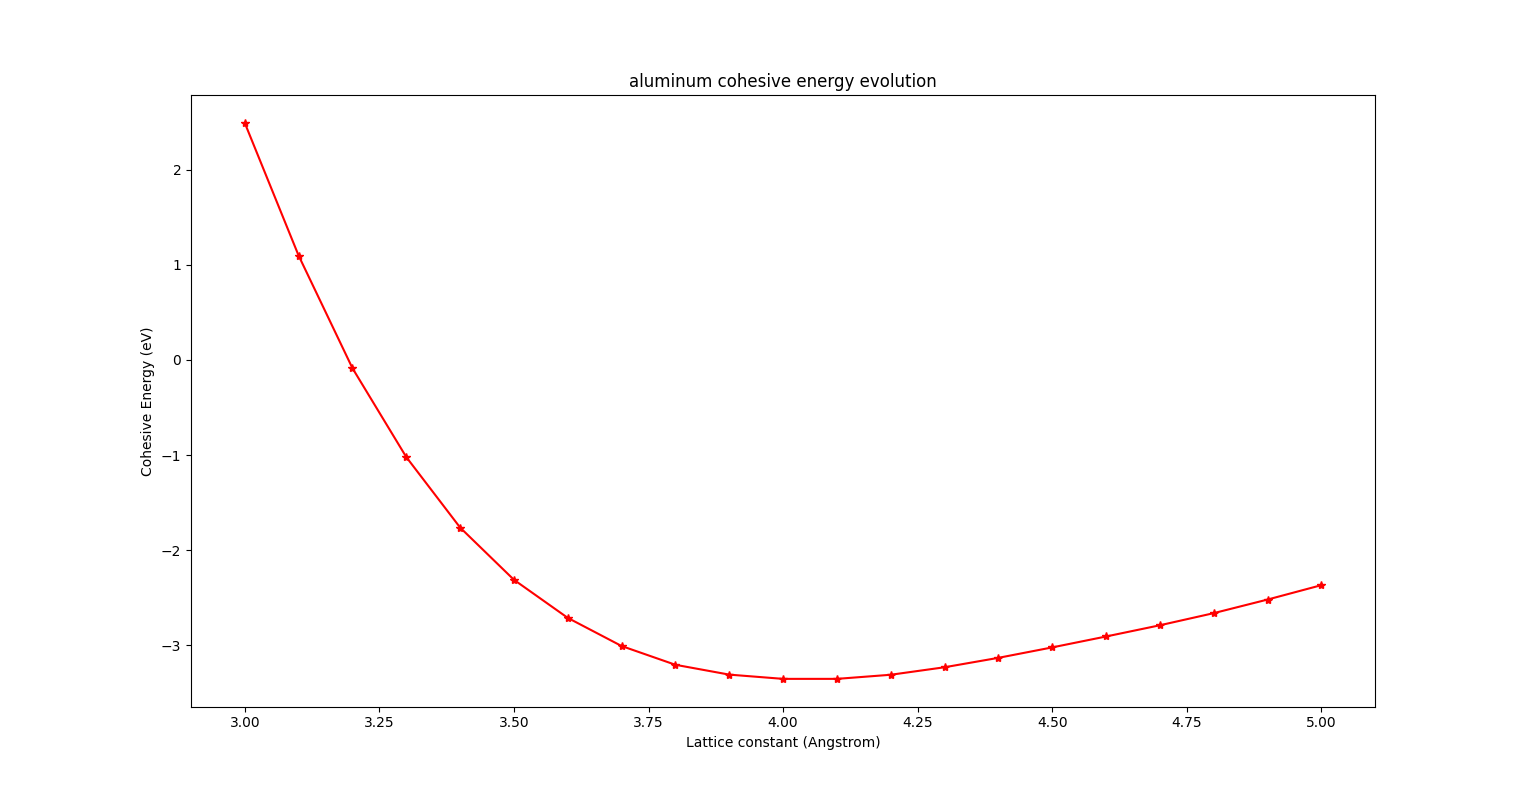
\includegraphics[height=2.50in,width=4.0in, viewport=0 0 1050 554,clip]{Lammps-EOS.png}
\caption{\fontsize{6.2pt}{5.2pt}\selectfont{\textrm{Aluminum cohesive energy evolution.}}}%(与文献\cite{EPJB33-47_2003}图1对比)
\label{LAMMPS_output-EOS}
\end{figure}
}

\frame[allowframebreaks]
{
	\frametitle{\textrm{LAMMPS}的输入文件}
	{\fontsize{6.0pt}{4.0pt}\selectfont{
%\verbatiminput{Figures/Lammps_in_lj.txt} %为保险:~选用文件名绝对路径
\verbatiminput{Figures/Lammps_tutorial-03-Lammps-in.txt} %为保险:~选用文件名绝对路径
}}
}

\frame[allowframebreaks]
{
	\frametitle{\textrm{LAMMPS}的输入文件:~基于\textrm{Matlab}的执行}
	{\fontsize{6.0pt}{4.0pt}\selectfont{
%\verbatiminput{Figures/Lammps_in_lj.txt} %为保险:~选用文件名绝对路径
\verbatiminput{Figures/Lammps_tutorial-03-Matlab-in.txt} %为保险:~选用文件名绝对路径
}}
}

\frame[allowframebreaks]
{
	\frametitle{\textrm{LAMMPS}的输入文件:~基于\textrm{Python}的执行}
	{\fontsize{6.0pt}{4.0pt}\selectfont{
%\verbatiminput{Figures/Lammps_in_lj.txt} %为保险:~选用文件名绝对路径
\verbatiminput{Figures/Lammps_tutorial-03-Python-in.txt} %为保险:~选用文件名绝对路径
}}
}

\frame
{
	\frametitle{应力-应变曲线}
\begin{figure}[h!]
\centering
\vskip -5pt
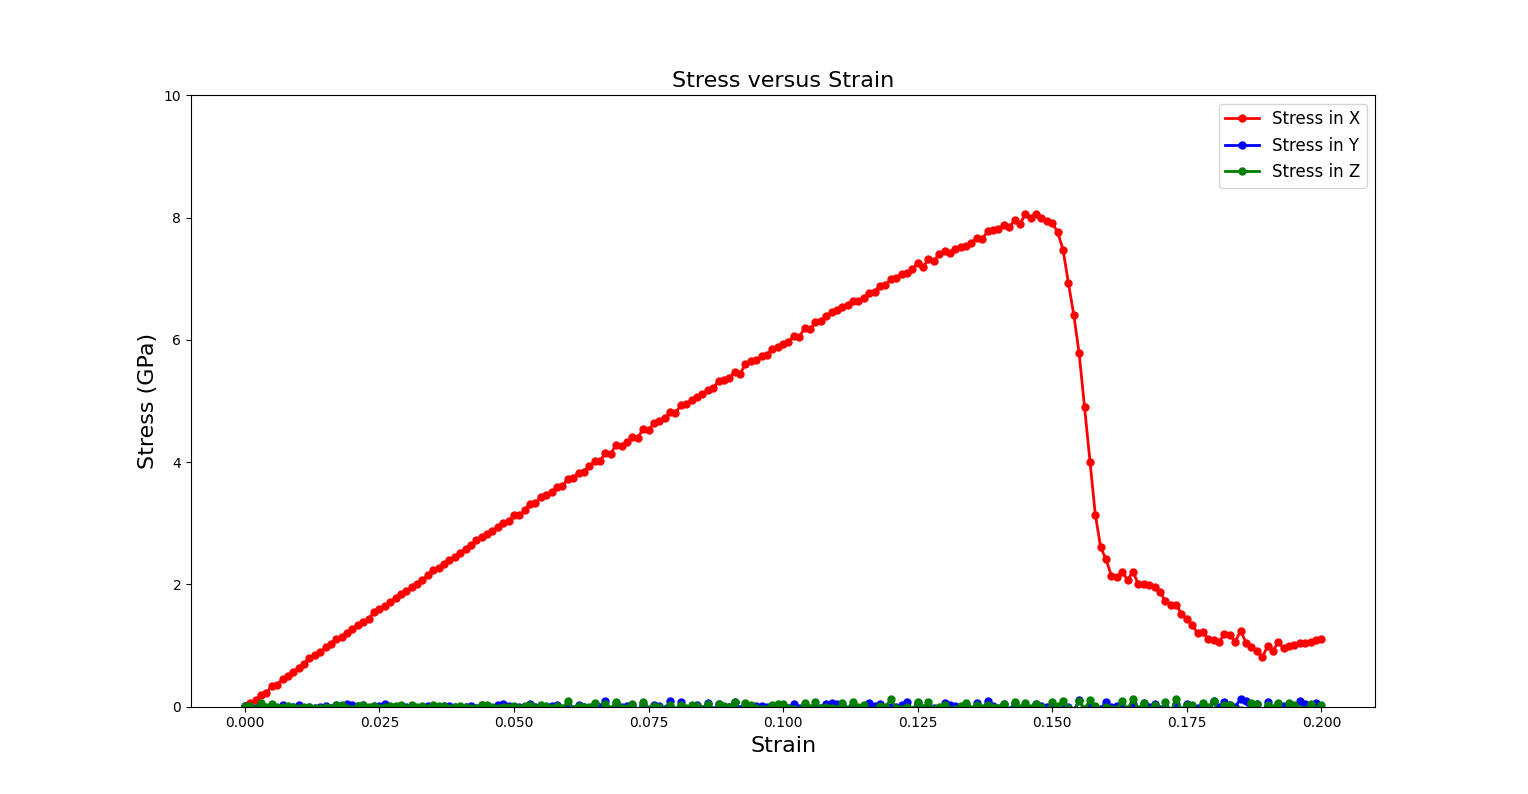
\includegraphics[height=2.20in,width=4.0in, viewport=0 0 1050 554,clip]{Lammps-Stress_Strain.png}
\caption{\fontsize{6.2pt}{5.2pt}\selectfont{\textrm{Stress-strain curve for uniaxial tensile loading of single crystal aluminum in the <100> loading direction.}}}%(与文献\cite{EPJB33-47_2003}图1对比)
\label{LAMMPS_output-Stress-Strain}
\end{figure}
}

\frame
{
	\frametitle{拉伸载荷}
\begin{figure}[h!]
\centering
\vskip -5pt
\animategraphics[autoplay, loop, height=2.40in, width=2.50in,viewport= 0 0 256 256,clip]{1}{Figures/Lammps-simulation-cell-in-tension-}{0}{81}
\caption{\fontsize{6.2pt}{5.2pt}\selectfont{\textrm{Tensile Loading of an Aluminum Single Crystal..}}}%(与文献\cite{EPJB33-47_2003}图1对比)
\label{LAMMPS_Tensile-Loading}
\end{figure}
}
%\vskip 5pt
%\frame
%------------------------------------------------------------------------Reference----------------------------------------------------------------------------------------------
		\frame[allowframebreaks]
{
\frametitle{主要参考文献}
\begin{thebibliography}{99}
{\tiny
	\bibitem{J.-G._Lee}\textrm{J.-G. Lee, \textit{Computational Materials Science:~an introduction}}~\textrm{(2nd Edition),~CPC Press}, \textrm{(2017)}
	\bibitem{url_lammps-tutorials}\url{https://github.com/mrkllntschpp/lammps-tutorials}
}
\end{thebibliography}
}
